Machine learning is concerned with the development of statistical algorithms that can \enquote{learn} from data and generalize to unseen data, without being explicitly programmed. One particular class of such algorithms is \emph{neural networks}, originally inspired by the human brain, which have proven highly successful. 
Technically, these fall under \emph{deep learning}, which is a subset of machine learning. Still, the use of deep-learning methods has become so ubiquitous (at least in physics applications) that both these terms are used more or less synonymously. 

Machine learning requires large-scale matrix computations. These can be performed efficiently on graphics processing units (GPUs). This thesis makes use of \emph{PyTorch}~\cite{paszke2019pytorchimperativestylehighperformance}, which is Python-based, to handle these computations. PyTorch also serves as an extensive machine-learning library, which includes models, loss functions and optimizers.
The hardware used in this thesis is provided by the HPC cluster PALMA II of the University of Münster.

% -- thesis motivation --
% use machine learning
% focus only on BBHs because BNS complicate searches in two ways:
% day long -> source moves on the sky
% multi-messenger -> need for negative latency alert
% focus on long signals first
% then overlapping

The investigation of machine-learning methods to complement matched filtering, for low-latency searches in particular, is not novel \cite{George_2018}. Recently, the increased amount of data from the growing second-generation GW observatory network, and the corresponding computational burden has motivated such studies \cite{PhysRevD.100.063015}. The research focuses primarily on convolutional neural networks (CNNs), and finds comparable performance while being far more computationally efficient, which is important for real-time detection.

This chapter introduces the basics of machine learning. This includes artificial neurons, how they are arranged into neural networks, and how these networks are trained to extract relevant information from data. Two architectures will be presented in detail, CNNs and the Transformer~\cite{NIPS2017_3f5ee243}.

\section{Basics}

\begin{figure}
	\centering
	\makebox[\textwidth]{
		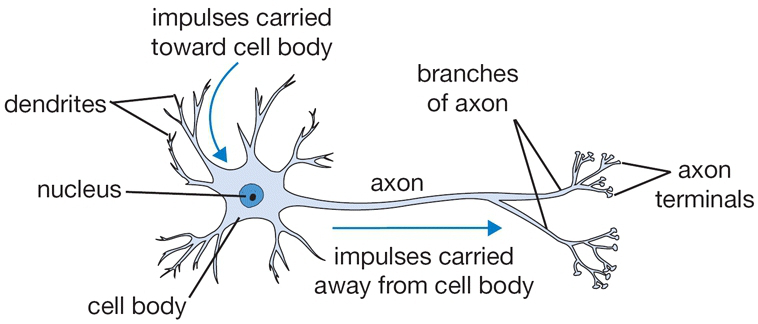
\includegraphics[width=8.5cm,align=c]{machine_learning/images/stanford_neuron}
		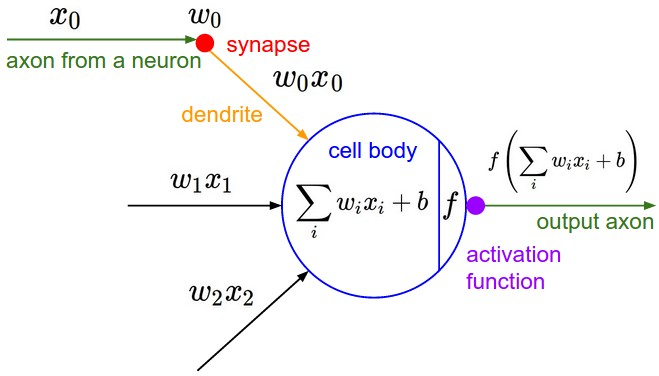
\includegraphics[width=8.5cm,align=c]{machine_learning/images/stanford_perceptron}
	}
	\caption{Drawing of a biological neuron (\emph{left}) and the mathematical model of an artificial neuron (\emph{right}). Taken from \cite{cs231n_neural_networks}.}
	\label{fig:machine_learning:neuron}
\end{figure}

% biological neuron -> artificial neuron
The fundamental building blocks of neural networks are \emph{artificial neurons}. 
These were originally conceived as simplified models of \emph{biological} neurons, excitable nerve cells in the brain, which receive and transmit electrical signals. Such cells consist of multiple dendrites, which carry signals towards the cell body, and one single axon that carries nerve signals away from it. The axon branches into a number of axon terminals, which transmit signals via synapses to the dendrites of other nerve cells. See a drawing in Fig.~\ref{fig:machine_learning:neuron} on the left.

Artificial neurons model this behavior by taking a number of inputs $\vec{x}$, \emph{e.g.}, from other neurons, for which they produce a single output $y$. The neuron assigns weights to each input, modeling the synaptic strength between itself and previous neurons. These weights $\vec{w}$ are \enquote{learnable}, and can be positive (excitatory) or negative (inhibitory). Initial research modeled neurons to always have a binary output, \emph{e.g.} $0$ or $1$. The neuron sums all weighted inputs, and \enquote{fires} if that sum exceeds a certain threshold $t$:
\begin{equation}
	y = \begin{cases}
		1 & \text{if } \vec{x}\cdot\vec{w} > t, \\
		0 & \text{else.}
	\end{cases}
\end{equation}
Artificial neurons were later modified to produce a continuous output, 
\begin{equation}
	y = f(\vec{x}\cdot\vec{w} + b), 
\end{equation}
with the addition of a learnable bias $b$, and the inclusion of a non-linear \emph{activation function} $f$. A common choice for this function is the rectified linear unit, $\text{ReLU}(z) = \max(0, z)$. 
Notice that both these equations are equivalent if $b=-t$ and $f$ is a step function.
Fig.~\ref{fig:machine_learning:neuron} shows a schematic of the artificial neuron, and how it relates to its biological counterpart.

\begin{figure}
	\centering
	\makebox[\textwidth]{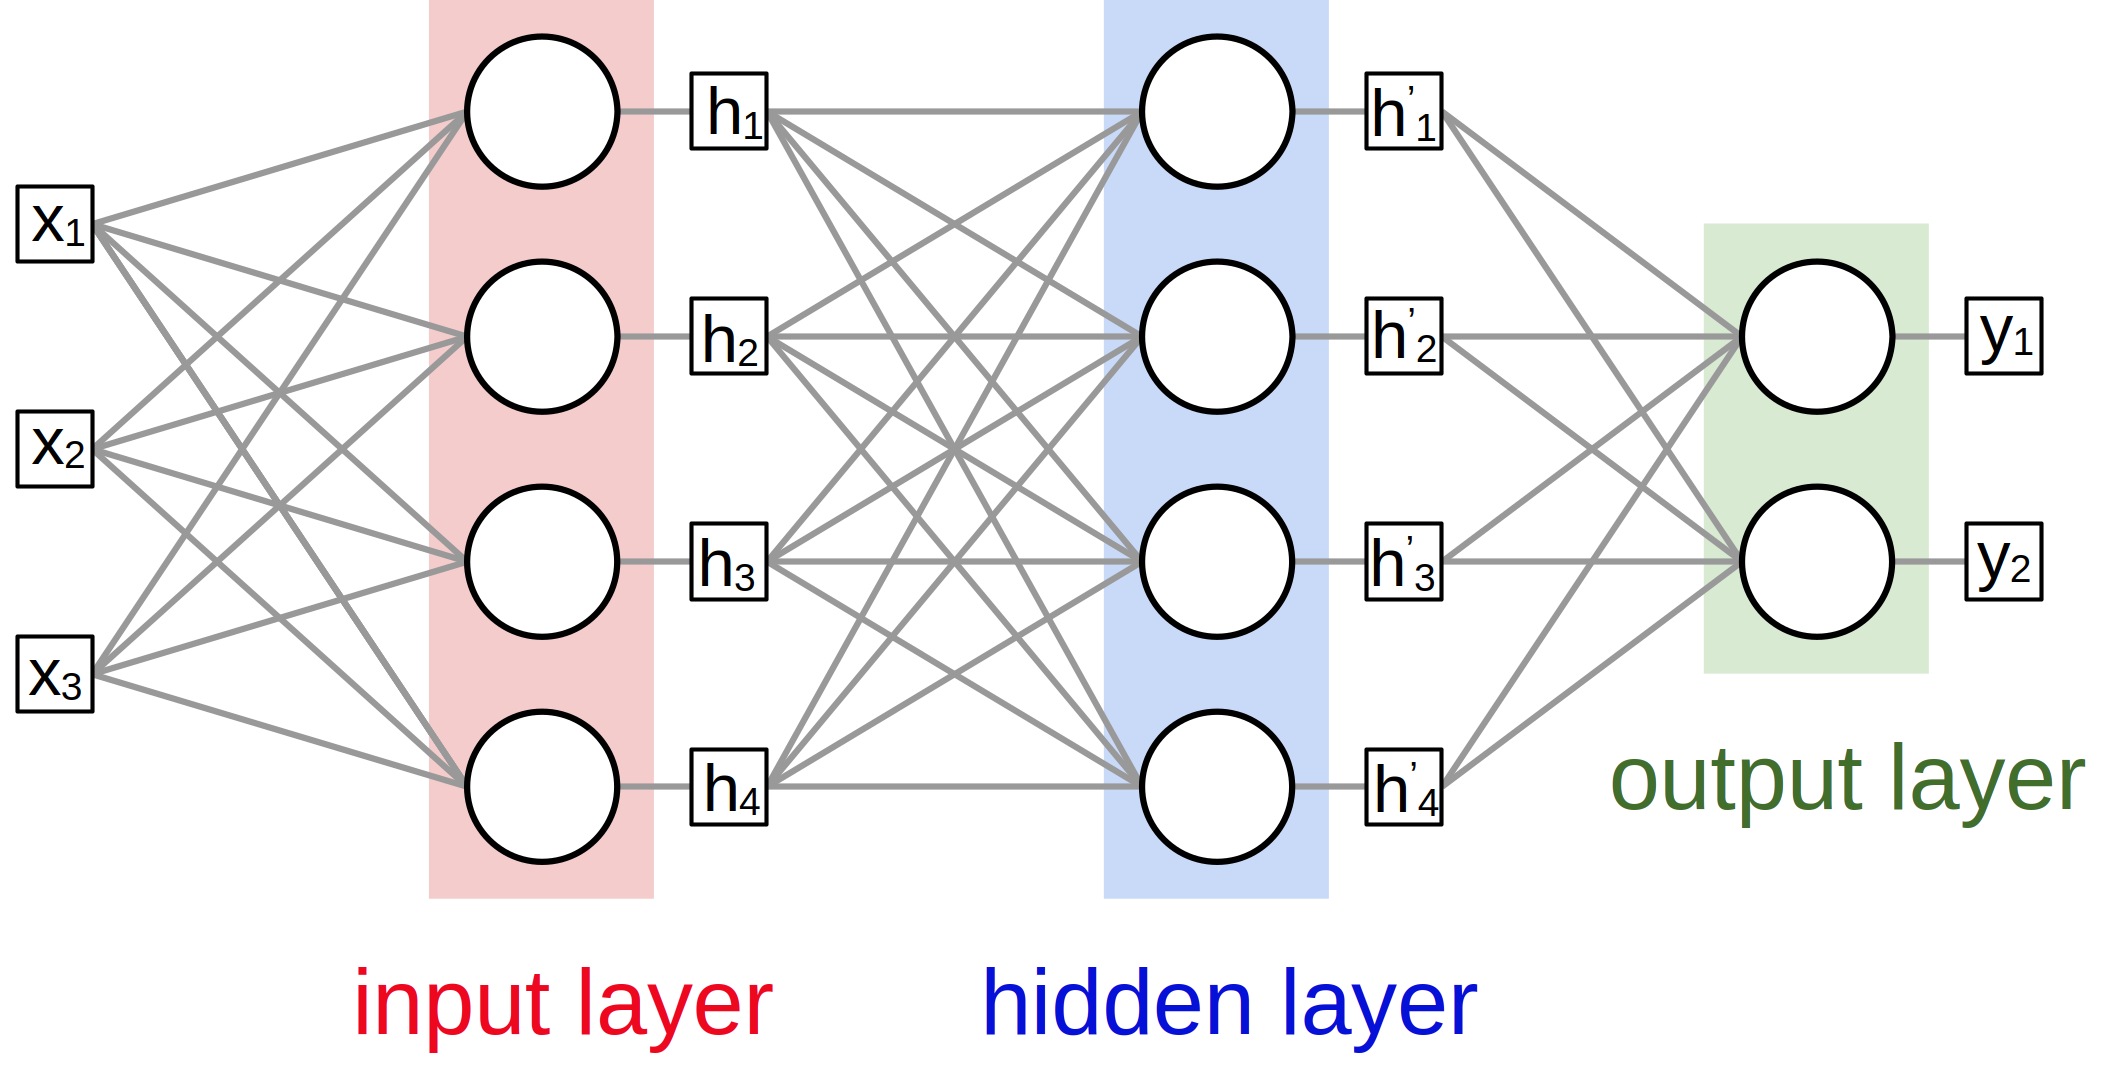
\includegraphics[width=11cm]{machine_learning/images/mlp}}
	\caption{A dense neural network with three layers. Each dot denotes an artificial neuron. The network takes an input $\vec{x}$ and projects it to $\vec{h}$, and then $\vec{h}'$, of hidden dimension four. The final output layer projects $\vec{h}'$ to $\vec{y}$.}
	\label{fig:machine_learning:mlp}
\end{figure}

% neurons arranged into fully connected layer 
% multiple layers form a neural network, a fully connected network (FCN) or dense network
% commonly this type of network is also called MLP, which is a misnomer, or FFN

These neurons can be arranged to form \emph{fully connected} or \emph{dense} layers. Such a layer takes $m$ inputs $\vec{x}$, and returns $n$ outputs $\vec{y}$, corresponding to the number of neurons. Each neuron is connected to all inputs, hence the name. Denoting the layer's weights $W_{m\times n}$ and the biases $\vec{b}$, this can be formalized as,
\begin{equation}
	\label{eq:machine_learning:dense_layer}
	\vec{y} = f(\vec{x}\,W_{m\times n} + \vec{b}).
\end{equation}
The term $\vec{x}\,W_{m\times n} + \vec{b}$ is conventionally called a \emph{linear projection} from the input dimension $m$ to the output dimension $n$, and it will be notated as $\text{Linear}_{m\rightarrow n}(\vec{x})$ in this thesis. The whole layer performs a non-linear projection then.

Stacking dense layers yields a fully connected or a dense neural network, which consists of one input layer, a number of hidden layers, and an output layer. Each layer's output corresponds to the next layer's input.  See a schematic in Fig.~\ref{fig:machine_learning:mlp}.
Stacked layers illustrate the importance of \emph{non-linear} activation functions, since without them, multiple layers would be equivalent to a single layer. 
Dense networks are commonly called multi-layer perceptrons (MLPs) or feed forward networks (FFNs).

% training
% dataset of labeled samples (supervised learning)
% training, validation, testing
% objective: minimize loss function L_L2 = sum (y_i-ŷ_i)²
% gradient descent 
% backpropagation
% batches

Having presented the basic form of a neural network, the question remains how its parameters should be chosen for the network to perform some specific task on a dataset. For a given dataset \emph{sample} $x$, the network makes a \emph{prediction} $\hat{y}$, which ideally corresponds to the true \emph{target} value $y$. In the context of GW searches, the input may be detector data, and the network predicts $1$ if that data contains a GW signal and $0$ otherwise. 

\begin{figure}
	\centering
	\makebox[\textwidth]{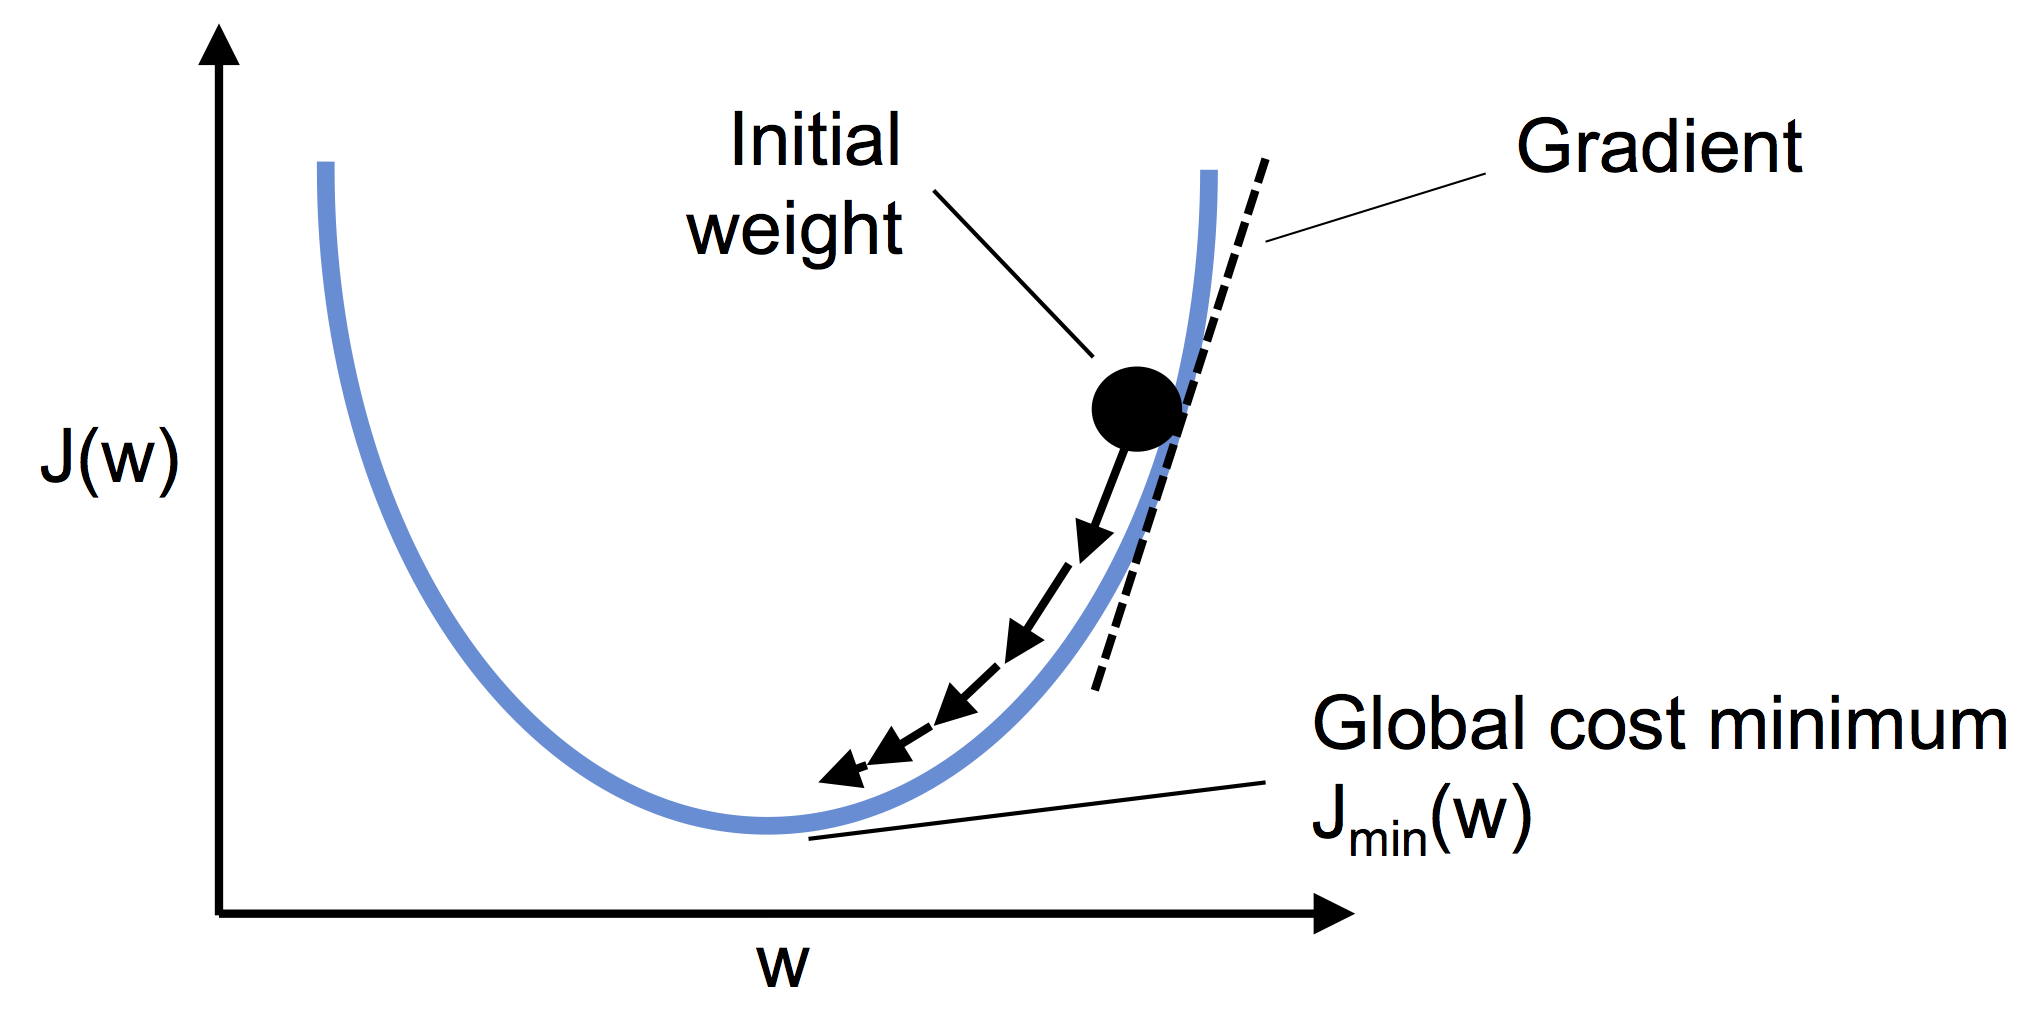
\includegraphics[width=10cm]{machine_learning/images/gradient_descent}}
	\caption{Gradient descent minimization of the loss $J$ with respect to the network parameters or weights $w$. This is a simplified sketch, where $w$ is one-dimensional. Contrast this with modern large language models with billions of parameters. Taken from \cite{raschka}.}
	\label{fig:machine_learning:gradient_descent}
\end{figure}

The process of optimizing a network's parameters is called \emph{training}. In particular, this thesis is concerned with \emph{supervised} learning, where this dataset is labeled, \emph{i.e.} the true values are known. In this case, the dataset is split into training, validation and testing subsets. The parameters are optimized by  minimizing a \emph{loss function} $\pazocal{L}$ over the training set, \emph{e.g.}, the mean-squared loss,
\begin{equation}
	\pazocal{L}_\text{MSE} = \frac{1}{N}\sum_{i=1}^{N}|\hat{y}(x_i, \vec{\theta}) - y_i|^2, 
\end{equation}
where $N$ is the number of training samples.
Notice that the total loss depends solely on the network parameters $\vec{\theta}$. Formally, the optimal parameters are given by,
\begin{equation}
	\vec{\theta}_\text{opt} = \argmin_{\vec{\theta}}
	\pazocal{L}(\vec{\theta}).
\end{equation}
Determining the minimum of $\pazocal{L}$ analytically is not possible once the model reaches a certain size. Instead, the parameters are initialized randomly and iteratively updated by calculating the gradient:
\begin{equation}
	\vec{\theta}' = \vec{\theta} - \eta\,\vec{\nabla}\pazocal{L}(\vec{\theta}),
\end{equation}
where $\eta$ denotes the \emph{learning rate}. This method is called \emph{gradient descent}. The parameters follow the slope of the loss hypersurface towards its minimum (see Fig.~\ref{fig:machine_learning:gradient_descent}). The loss gradient can be efficiently computed with \emph{backpropagation}, which is simply based on the chain rule.

In practice, it is often not feasible or even necessary to update the parameters based on the loss of the whole training dataset. Instead, small batches are chosen randomly, for which the parameters are updated subsequently. Once the whole dataset is exhausted, the process is repeated. One full iteration over the training dataset is called an \emph{epoch}.

% loss vs epochs -> learning curve -> overfit, underfit
% regularization
% dropout, lambda, decrease model size, increase number of samples

\section{Convolutional Neural Networks}

\begin{figure}
	\centering
	\makebox[\textwidth]{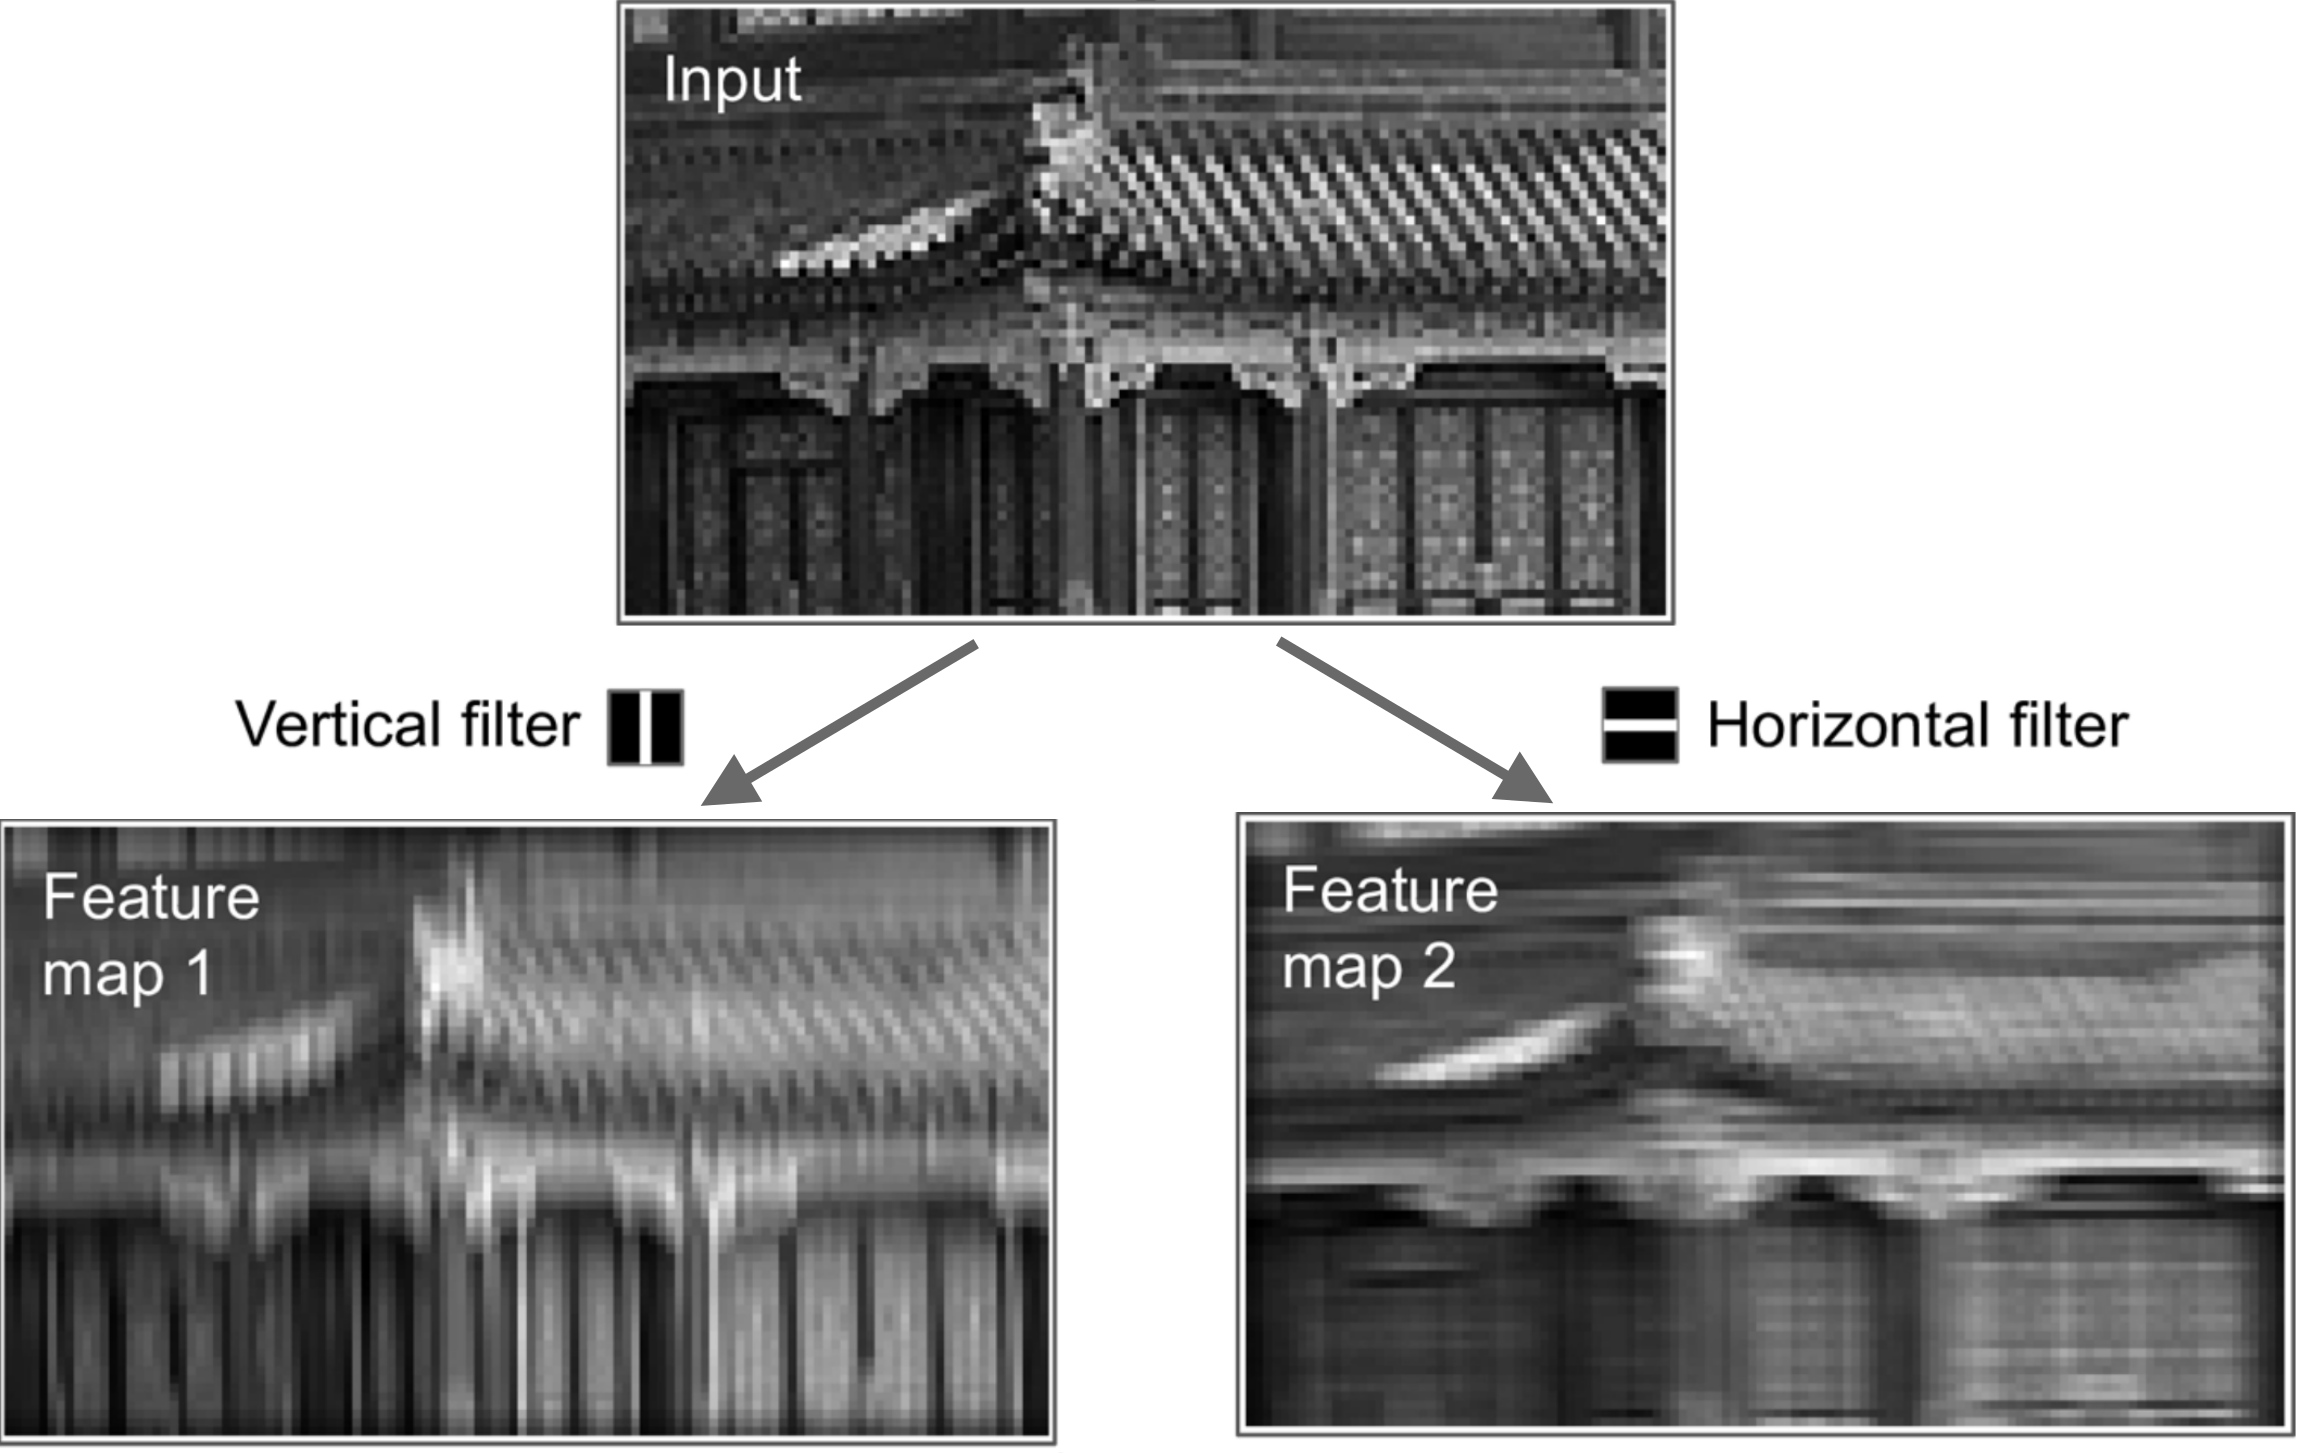
\includegraphics[width=11cm]{machine_learning/images/cnn/filter.png}}
	\caption{A \enquote{vertical} and a \enquote{horizontal} filter convolved over the image of a pagoda. In the feature map on the left, the vertical features stand out more. \emph{e.g.} the roof tiles and the columns. On the right they appear less bright and more blurry. Adapted from \cite{hands_on_ml}.}
	\label{fig:machine_learning:convolution}
\end{figure}

% Visual cortex -> conv operation (similarity to matched filtering) (explaing padding)

CNNs were first developed for image analysis and were inspired by the organization of neurons in the brain's visual cortex \cite{hands_on_ml}. In the visual cortex, neurons have a \enquote{small} receptive field, that is, they respond only to local regions of the visual field. The receptive fields of different neurons can overlap and together they cover the whole visual field. Moreover, neurons can specialize to recognize different local patterns, such as horizontal and vertical edges. 

CNNs model this behavior by convolving learnable filters, called \emph{kernels}, across the input. In practice, this operation is usually implemented as the cross-correlation between a kernel $k$ and an input $x$. In one dimension, this is given by
\begin{equation}
	(k\star x)(\tau) = \int_\mathbb{R}\mathrm{d}t\, k(t)\,x(t+\tau),
\end{equation}
and yields a measure of similarity as a function of $\tau$, the displacement of the input relative to the kernel. 
In discrete form, the convolution of a kernel $\vec{k}$ of size $N$ over an input $\vec{x}$ outputs a \emph{feature map} $\vec{y}$ with entries
\begin{equation}
	y_i = (\vec{k}\star\vec{x})_i = \sum_{j=0}^{N-1} k_j\,x_{i+j}.
\end{equation}
See Fig.~\ref{fig:machine_learning:convolution}, where two different kernels are applied to the same input image of a pagoda. One kernel extracts the input's vertical features, while the other extracts horizontal features.
The convolution operation gives neural networks the ability to extract features in a spatially invariant manner.
% TODO: more stuff about whats cool here

% explain CNN architecture:
% How do channels work
% Subsampling with pooling, stride

\begin{figure}
	\centering
	\makebox[\textwidth]{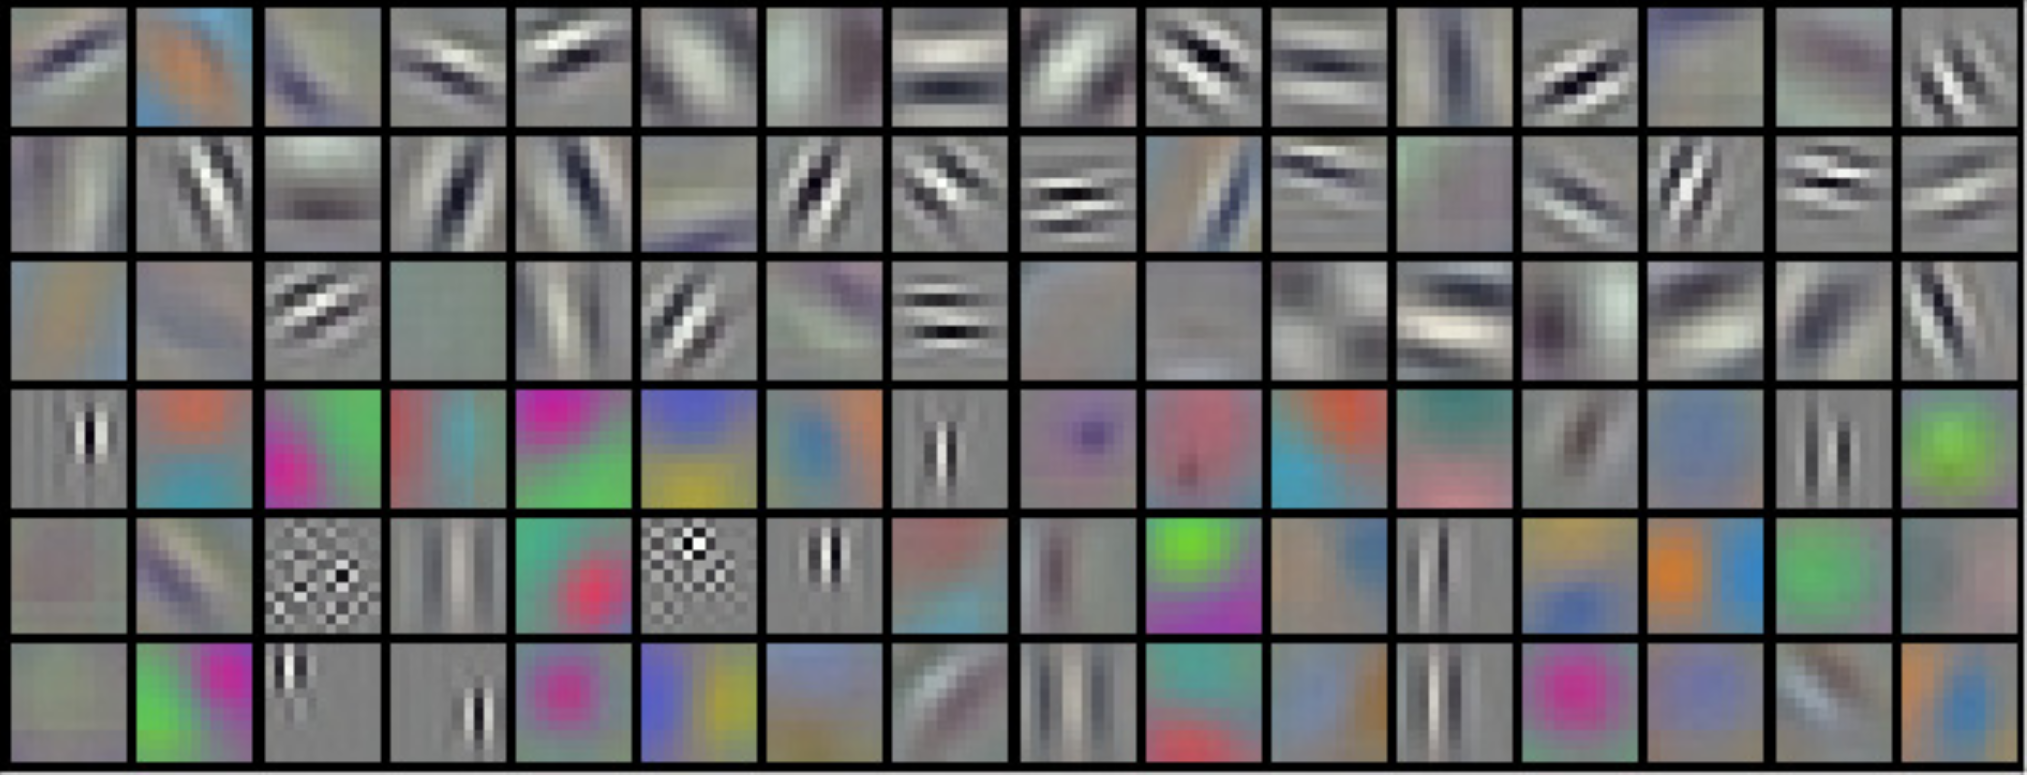
\includegraphics[width=10cm]{machine_learning/images/imagenet/kernels}}
	\caption{The initial convolutional layer's 96 kernels in AlexNet \cite{10.1145/3065386}. These are of shape $3\times11\times11$, and plotted as RGB images.}
	\label{fig:machine_learning:kernels}
\end{figure}

\begin{figure}
	\centering
	\makebox[\textwidth]{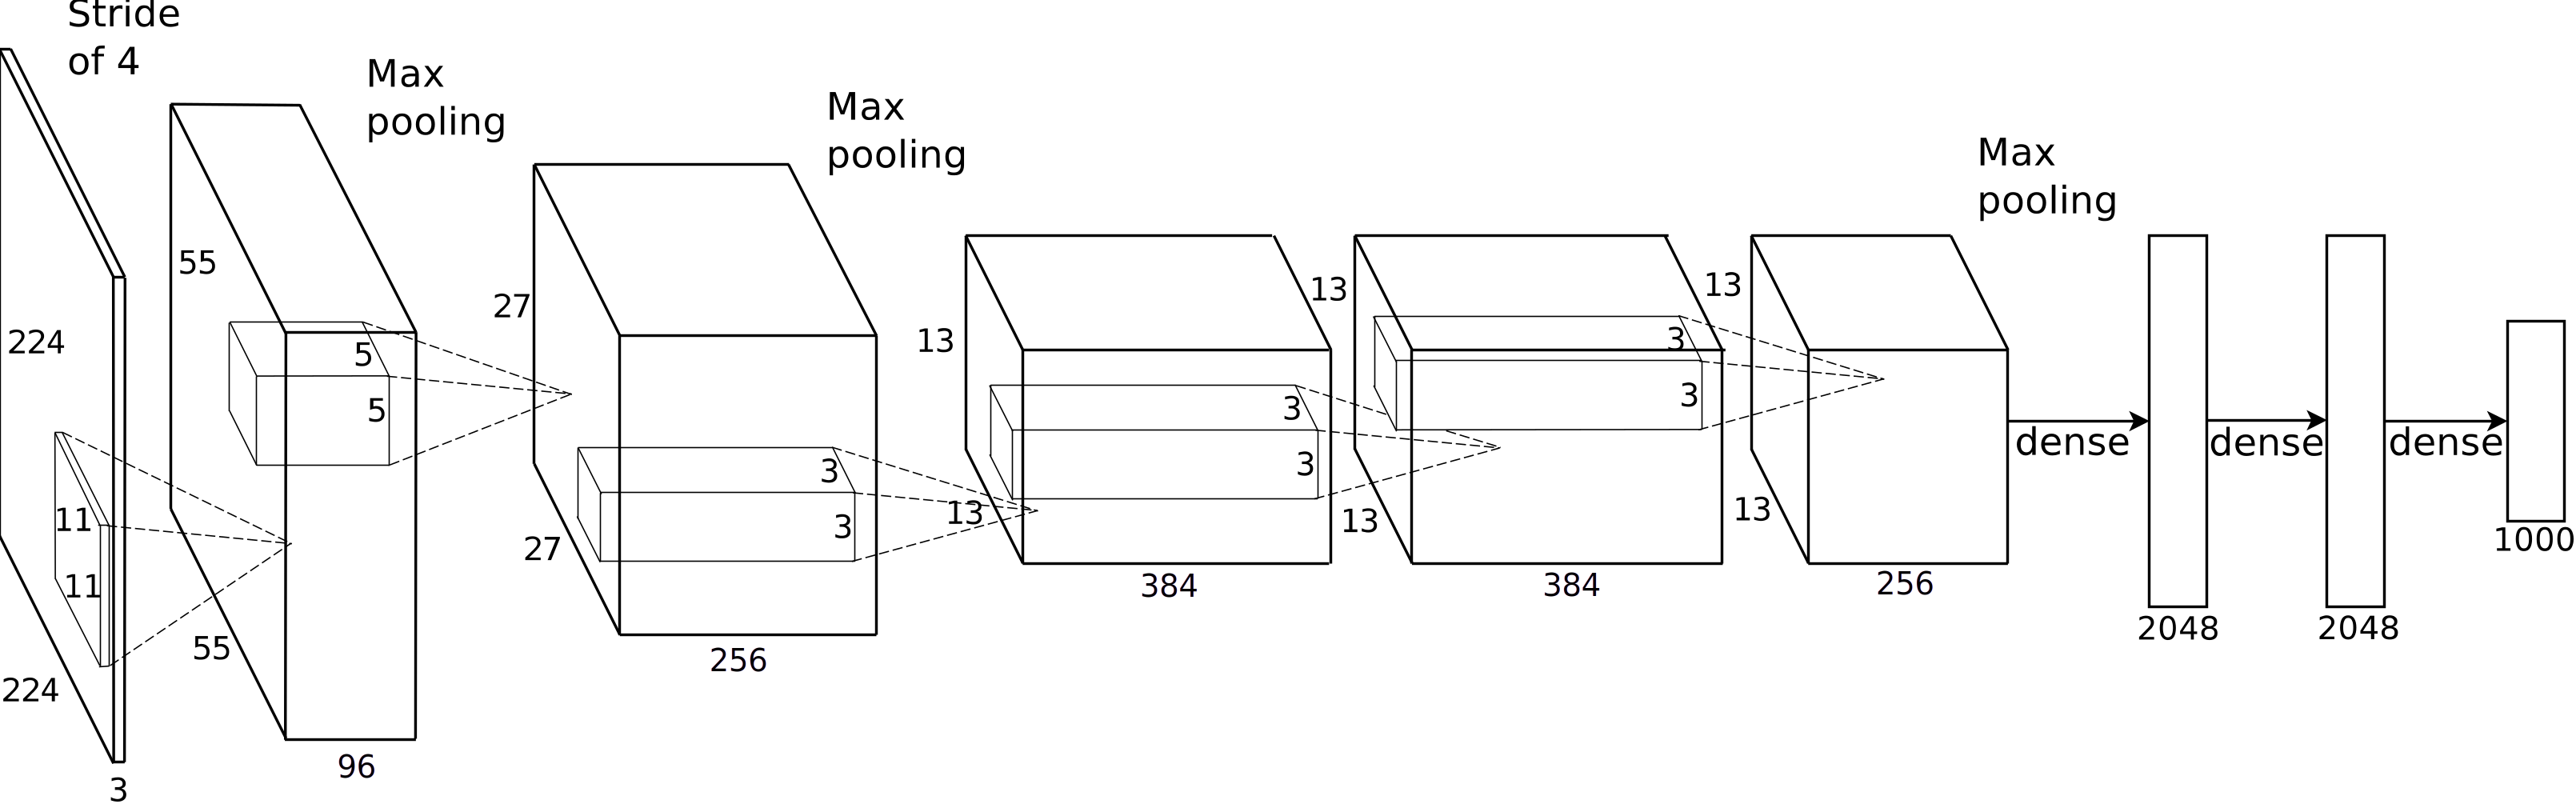
\includegraphics[width=17cm]{machine_learning/images/imagenet/Krizhevsky-2012.png}}
	\caption{AlexNet architecture \cite{10.1145/3065386}. Multiple stacked convolutional layers with ReLU and pooling in between, and a final dense network. The schematic has been adapted.}
	\label{fig:machine_learning:cnn}
\end{figure}

A full CNN architecture will consist of multiple stacked \emph{convolutional layers}. Each layer learns a number of kernels producing multiple feature maps, or \emph{channels}. One layer's output gets fed to the next layer.
This way, the complexity of the features that are extracted from the input gradually increases. 
The initial layers will learn low-level features, \emph{e.g.} vertical or horizontal edges, while the later layers can extract high-level features, \emph{e.g.} human faces or GW signals. See the learned low-level kernels of a 2D-CNN, AlexNet \cite{10.1145/3065386}, in Fig.~\ref{fig:machine_learning:kernels}. 

Generally, a 1D convolutional layer takes an input tensor $X$ of shape $C_\text{in} \times L$ and produces an output of shape $C_\text{out} \times L$. The sequence length is $L$, and $C_\text{in}$ and $C_\text{out}$ denote the number of input and output channels. The output of such a layer is then,
\begin{equation}
	\text{ConvLayer}_{C_\text{in}\rightarrow C_\text{out}}(X)
	= \concat_{i=0}^{C_\text{out}-1}\sum_{j=0}^{C_\text{in}-1} \vec{k}_{i,j}\star\vec{x}_j,
\end{equation}
with $\vec{k}_{i,j}$, the kernel corresponding to the $i$-th output channel and the $j$-th input channel.

Usually, the number of channels increases the deeper the CNN gets. To counteract the increased computational burden this introduces, CNNs often perform downsampling on the feature maps between each layer. This can be achieved by \emph{striding}, which disregards some of the feature map entries in an orderly fashion, \emph{e.g.} every second, which corresponds to a stride of two. Another way of downsampling is \emph{pooling}, where the feature map is subdivided into equal sized regions, and for each region only the maximum value or the mean value is extracted.

Most CNNs apply a number of convolutional layers, each followed by a ReLU non-linearity and downsampling. Without this non-linearity, multiple convolutional layers would be equivalent to a single layer, similar to stacked fully-connected layers. The final feature maps are usually flattened and fed to a fully-connected network to return an output of the desired size. See an example 2D-CNN in Fig.~\ref{fig:machine_learning:cnn}.

In GW signal detection, both two and one-dimensional CNNs are employed. In the former case, the network's input can be the strain spectrogram \cite{George_2018}, and in the latter case, it is the strain time series \cite{PhysRevD.100.063015}. Notice especially, the similarity of 1D-CNNs with matched filtering, which is based on \enquote{de-noising} the detector strain $s(t)$ with a filter function $K(t)$ via $\int\mathrm{d}tK(t)s(t)$ (see Eq.~\ref{eq:matched_filtering:filtered_strain}). In a way, the whole set of a CNN's kernel parameters can be thought of as a particularly efficient way of storing waveform templates.

\section{Transformers}
\label{sec:machine_learning:transformers}

% originally language processing, translation task
% also used in image or audio tasks
% based on attention

The Transformer \cite{NIPS2017_3f5ee243} was originally developed for natural language processing tasks (NLP), in particular for machine translation. 
Unlike CNNs, which rely on local receptive fields, Transformers model global dependencies through \emph{attention mechanisms}.
Transformers generalize well to other sequential data tasks, \emph{e.g.}\ image or audio related. A transformer-based model has proved successful in GW parameter estimation under ET conditions with signal overlap \cite{Papalini_2025}. This motivates the investigation of transformers for GW searches.

\subsection*{Attention Mechanism}

\begin{figure}
	\centering
	\makebox[\textwidth]{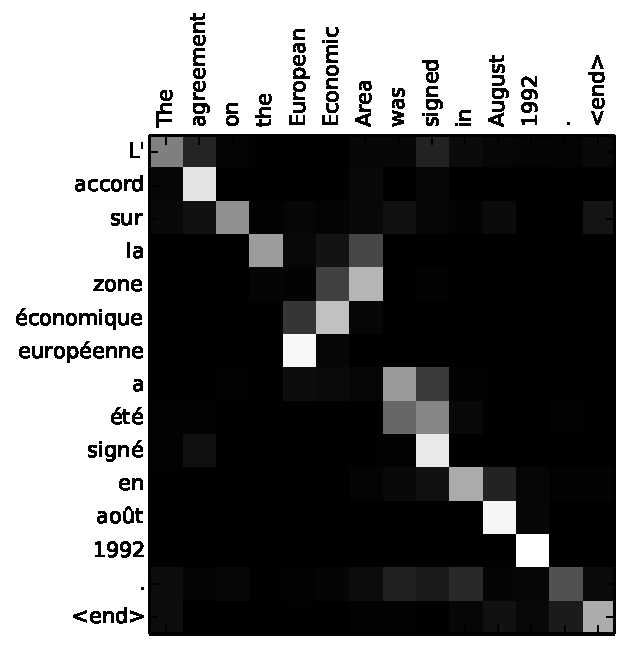
\includegraphics[width=8cm]{machine_learning/images/EEA}}
	\caption{Cross-attention matrix in an English-to-French translation model \cite{Bahdanau2014NeuralMT}. The English sentence is the source sequence, and the French translation the target sequence. Lighter colors mean higher values.}
	\label{fig:machine_learning:attn_matrix}
\end{figure}

The central component of the Transformer architecture is the attention mechanism, which builds on \cite{Bahdanau2014NeuralMT}. The mechanism takes two sequences as input. Each sequence comprises a number of tokens, which, \emph{e.g.}\ in NLP, can correspond to the words of a sentence. 
The two inputs are referred to as the \emph{source} sequence and the \emph{target} sequence. 
If both are the same, this is called \emph{self-attention}, and if they are different, it is \emph{cross-attention}. The attention mechanism relies on \emph{attention weights} to model the relationship between source and target sequence. These weights correspond to a $N_\text{tgt}\times N_\text{src}$ matrix. See an example in Fig.~\ref{fig:machine_learning:attn_matrix}, the attention matrix in an English-to-French translation model, capturing the relationship between  \enquote{area} in English and \enquote{zone} in French despite their different ordering in the two languages.

%\begin{figure}
%	\centering
%	\makebox[\textwidth]{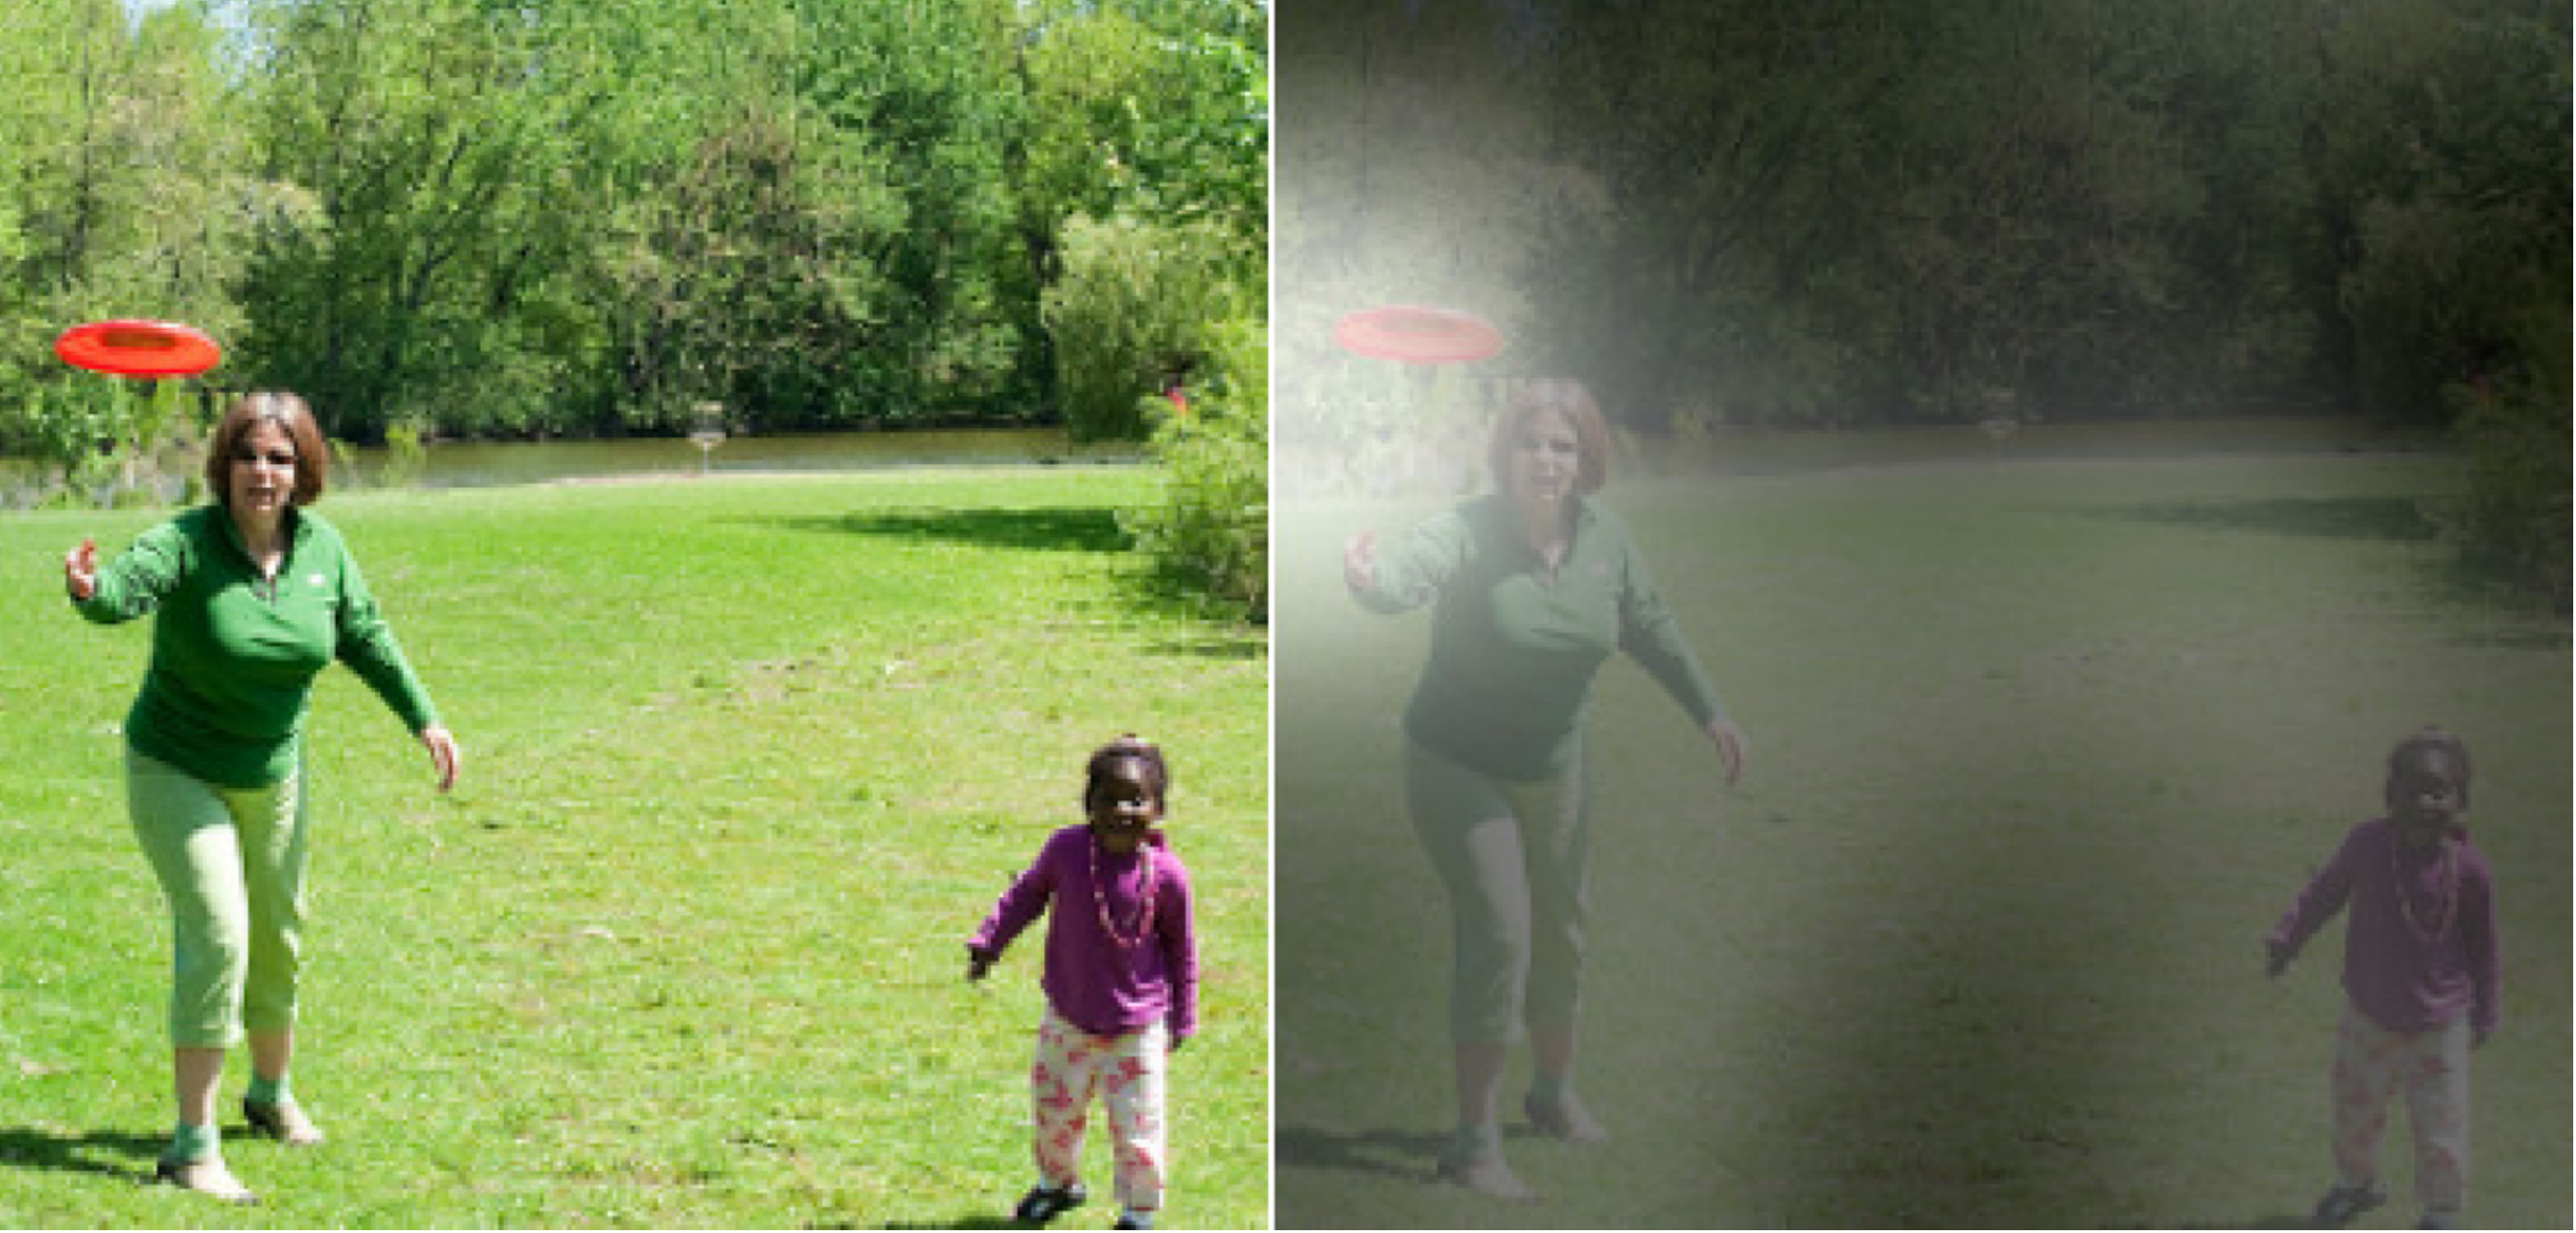
\includegraphics[width=13cm]{machine_learning/images/frisbee_attention}}
%	\caption{}
%	\label{fig:machine_learning:attention}
%\end{figure}

\subsection*{Scaled Dot-Product Attention}

In transformers, the attention mechanism is inspired by a search algorithm for a database of \emph{key}-\emph{value} pairs. The keys serve as identifiers and the values contain the actual data associated with them. The database is efficiently searched by matching a \emph{query} against the keys to retrieve the relevant values. 
For each query, the attention mechanism returns a weighted sum of all the values. The weights correspond to the similarity between the query and all keys, which is computed via their dot product.

This is implemented by linearly projecting the keys and values from the source sequence tokens, and the queries from the target sequence. The input tensors are denoted as $S_{N_\text{src}\times d_\text{src}}$ and $T_{N_\text{tgt}\times d_\text{tgt}}$, meaning source and target sequence respectively. Each sequence consists of a number of tokens $N$, which are vectors of size $d$. The queries, keys and values are then,
\begin{align}
	Q_{N_\text{tgt}\times d_\text{embed}} &= \text{Linear}_{d_\text{tgt} \rightarrow d_\text{embed}}(T) 
	\label{eq:machine_learning:q_proj} \\
	K_{N_\text{src}\times d_\text{embed}} &= \text{Linear}_{d_\text{src} \rightarrow d_\text{embed}}(S) 
	\label{eq:machine_learning:k_proj} \\
	V_{N_\text{src}\times d_\text{embed}} &= \text{Linear}_{d_\text{src} \rightarrow d_\text{embed}}(S)
	\label{eq:machine_learning:v_proj},
\end{align}
respectively, with the embedding dimension $d_\text{embed}$. (Notated like this, the linear projection only applies to the final tensor dimension, and its weights are shared across all other dimensions.)

From these, for each query vector $\vec{q}_i$, its weights $\vec{w}_i$ are computed as the dot product between that query vector and all keys:
\begin{equation}
	\vec{w}_i = \softmax\begin{pmatrix} 
		\vec{q}_i\cdot\vec{k}_0/\sqrt{d_\text{embed}} \\
		\vec{q}_i\cdot\vec{k}_1/\sqrt{d_\text{embed}} \\
		\vdots \\
		\vec{q}_i\cdot\vec{k}_{N_\text{src}-1}/\sqrt{d_\text{embed}}
	\end{pmatrix}.
\end{equation}
The dot product is scaled by the embedding dimension. \emph{Softmax} is applied to ensure that the weight vector sums to one. For an arbitrary vector $\vec{x}$ of size $N$ the softmax operation returns
\begin{equation}
	\softmax{\vec{x}} = \frac{1}{\sum_i \e^{x_i}} \begin{pmatrix}
		\e^{x_0} & \e^{x_1} & \dots & \e^{x_{N-1}}
	\end{pmatrix}^\intercal.
\end{equation}
The whole attention matrix has these weight vectors as its rows, \emph{i.e.},
\begin{equation}
	W_{N_\text{tgt}\times N_\text{src}} = \begin{pmatrix}
		\rule[0.5ex]{2.33em}{0.48pt}\;
		\vec{w}_0^\intercal 
		\,\rule[0.5ex]{2.33em}{0.48pt} \\
		\rule[0.5ex]{2.33em}{0.48pt}\; 
		\vec{w}_1^\intercal 
		\;\rule[0.5ex]{2.33em}{0.48pt} \\
		\vdots \\
		\rule[0.5ex]{1.5em}{0.48pt}\; 
		\vec{w}_{N_\text{tgt}-1}^\intercal 
		\;\rule[0.5ex]{1.5em}{0.48pt}
	\end{pmatrix}.
\end{equation}
Computing the attention weights as such is referred to as \emph{scaled dot-product attention}.

The attention mechanism will return a tensor of size $N_\text{tgt}\times d_\text{embed}$. To this end, the weight matrix and value tensor are multiplied. This yields a tensor, where each row is a weighted sum, $\sum_j w_{ij} \vec{v}_j$, corresponding to the $i$-th query. A final output linear projection is applied. The whole attention mechanism can be stated as,
\begin{equation}
	\label{eq:machine_learning:attn}
	\text{Attention}(Q, K, V) = \text{Linear}_{d_\text{embed} \rightarrow d_\text{embed}}(\softmax{\left(\frac{QK^\intercal}{\sqrt{d_\text{embed}}}\right)}\,V),
\end{equation}
with the attention matrix $W$ somewhat confusingly denoted as $\softmax{({QK^\intercal} / {\sqrt{d_\text{embed}}})}$, where softmax is applied along the final dimension.

Considering English-to-French machine-translation, the English sentence is the source sequence, while the target sequence somehow represents the French translation. (The correct translation is obviously not known beforehand. How the Transformer gains this representation will be covered later.) 
The projected values represent the English words in some abstract way, and the keys serve as labels for these values. Similarly, the query tokens are projected from the target sequence and encode what information is needed at each position. The French word corresponding to one of the queries is obtained by a weighted sum of all value tokens. The network learns to assign larger weights to the values most relevant to that position. A final linear layer projects this weighted sum of abstract English word representations into a French word representation.

\begin{figure}
	\centering
	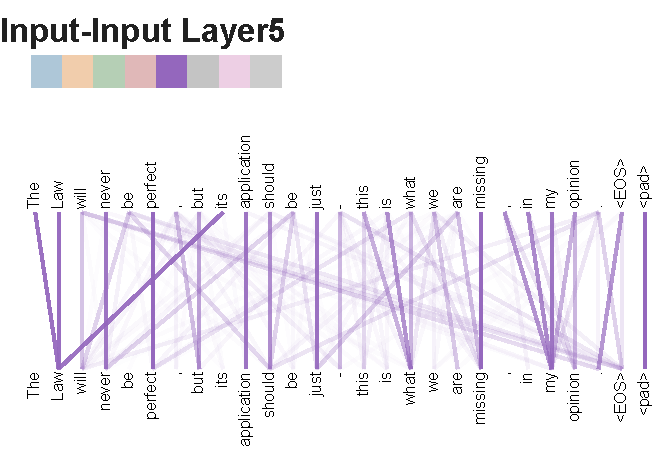
\includegraphics[
	width=10cm,
	trim=0cm 0cm 0cm 2cm,
	clip,
	angle=-90
	]{machine_learning/images/anaphora_resolution_new}
	\hspace{0.5em}
	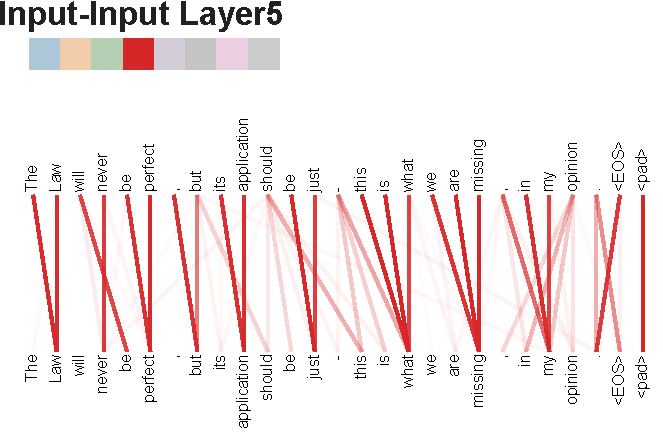
\includegraphics[
	width=10cm,
	trim=0cm 0cm 0cm 2cm,
	clip,
	angle=-90
	]{machine_learning/images/attending_to_head2_new}
	\hspace{0.5em}
	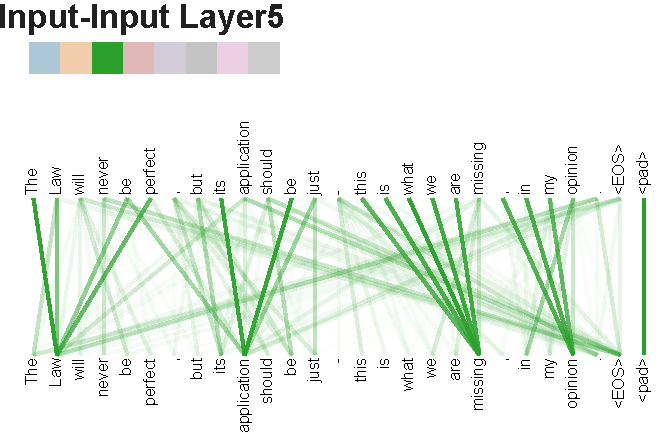
\includegraphics[
	width=10cm,
	trim=0cm 0cm 0cm 2cm,
	clip,
	angle=-90
	]{machine_learning/images/attending_to_head_new}
	\caption{Self-attention weights of different heads in the original Transformer \cite{NIPS2017_3f5ee243}.}
	\label{fig:machine_learning:mha}
\end{figure}

\subsection*{Multi-Head Attention}

Transformers develop the attention mechanism further to include multiple \emph{heads}. Each head learns its own query, key and value projections, and performs the attention mechanism independently of other heads. The idea is that each head can learn to perform different tasks (see Fig.~\ref{fig:machine_learning:mha}). This is called \emph{multi-head attention} (MHA).

In practice, to not introduce additional computational strain, the embedding dimension inside each head is reduced. This is usually implemented by keeping the original projections (Eqs.~\ref{eq:machine_learning:q_proj}, \ref{eq:machine_learning:k_proj}, \ref{eq:machine_learning:v_proj}), and splitting each tensor into $N_\text{heads}$ heads along the embedding dimension to yield tensors $Q_i$ of size $N_\text{tgt}\times d_\text{embed}/N_\text{heads}$ and $K_i$, $V_i$ of shape $N_\text{src}\times d_\text{embed}/N_\text{heads}$. For this to work, $d_\text{embed}$ has to be divisible by the total number of heads. The output of all heads is concatenated along their final dimension, and a linear projection is applied: 
\begin{equation}
	\text{MHA}(Q, K, V) 
	= \text{Linear}_{d_\text{embed} \rightarrow d_\text{embed}}
	{(\concat_{i=0}^{N_\text{heads}-1}
	{(\softmax{\left(\frac{Q_iK_i^\intercal}{\sqrt{{d_\text{embed}}/{N_\text{heads}}}}\right)}V_i)})}.
\end{equation}
Notice that for a single head, this is equivalent to Eq.~\ref{eq:machine_learning:attn}.

\subsection*{Model Architecture}

\begin{figure}
	\centering
	\begin{minipage}[t]{7cm}
		\centering
		\makebox[\textwidth]{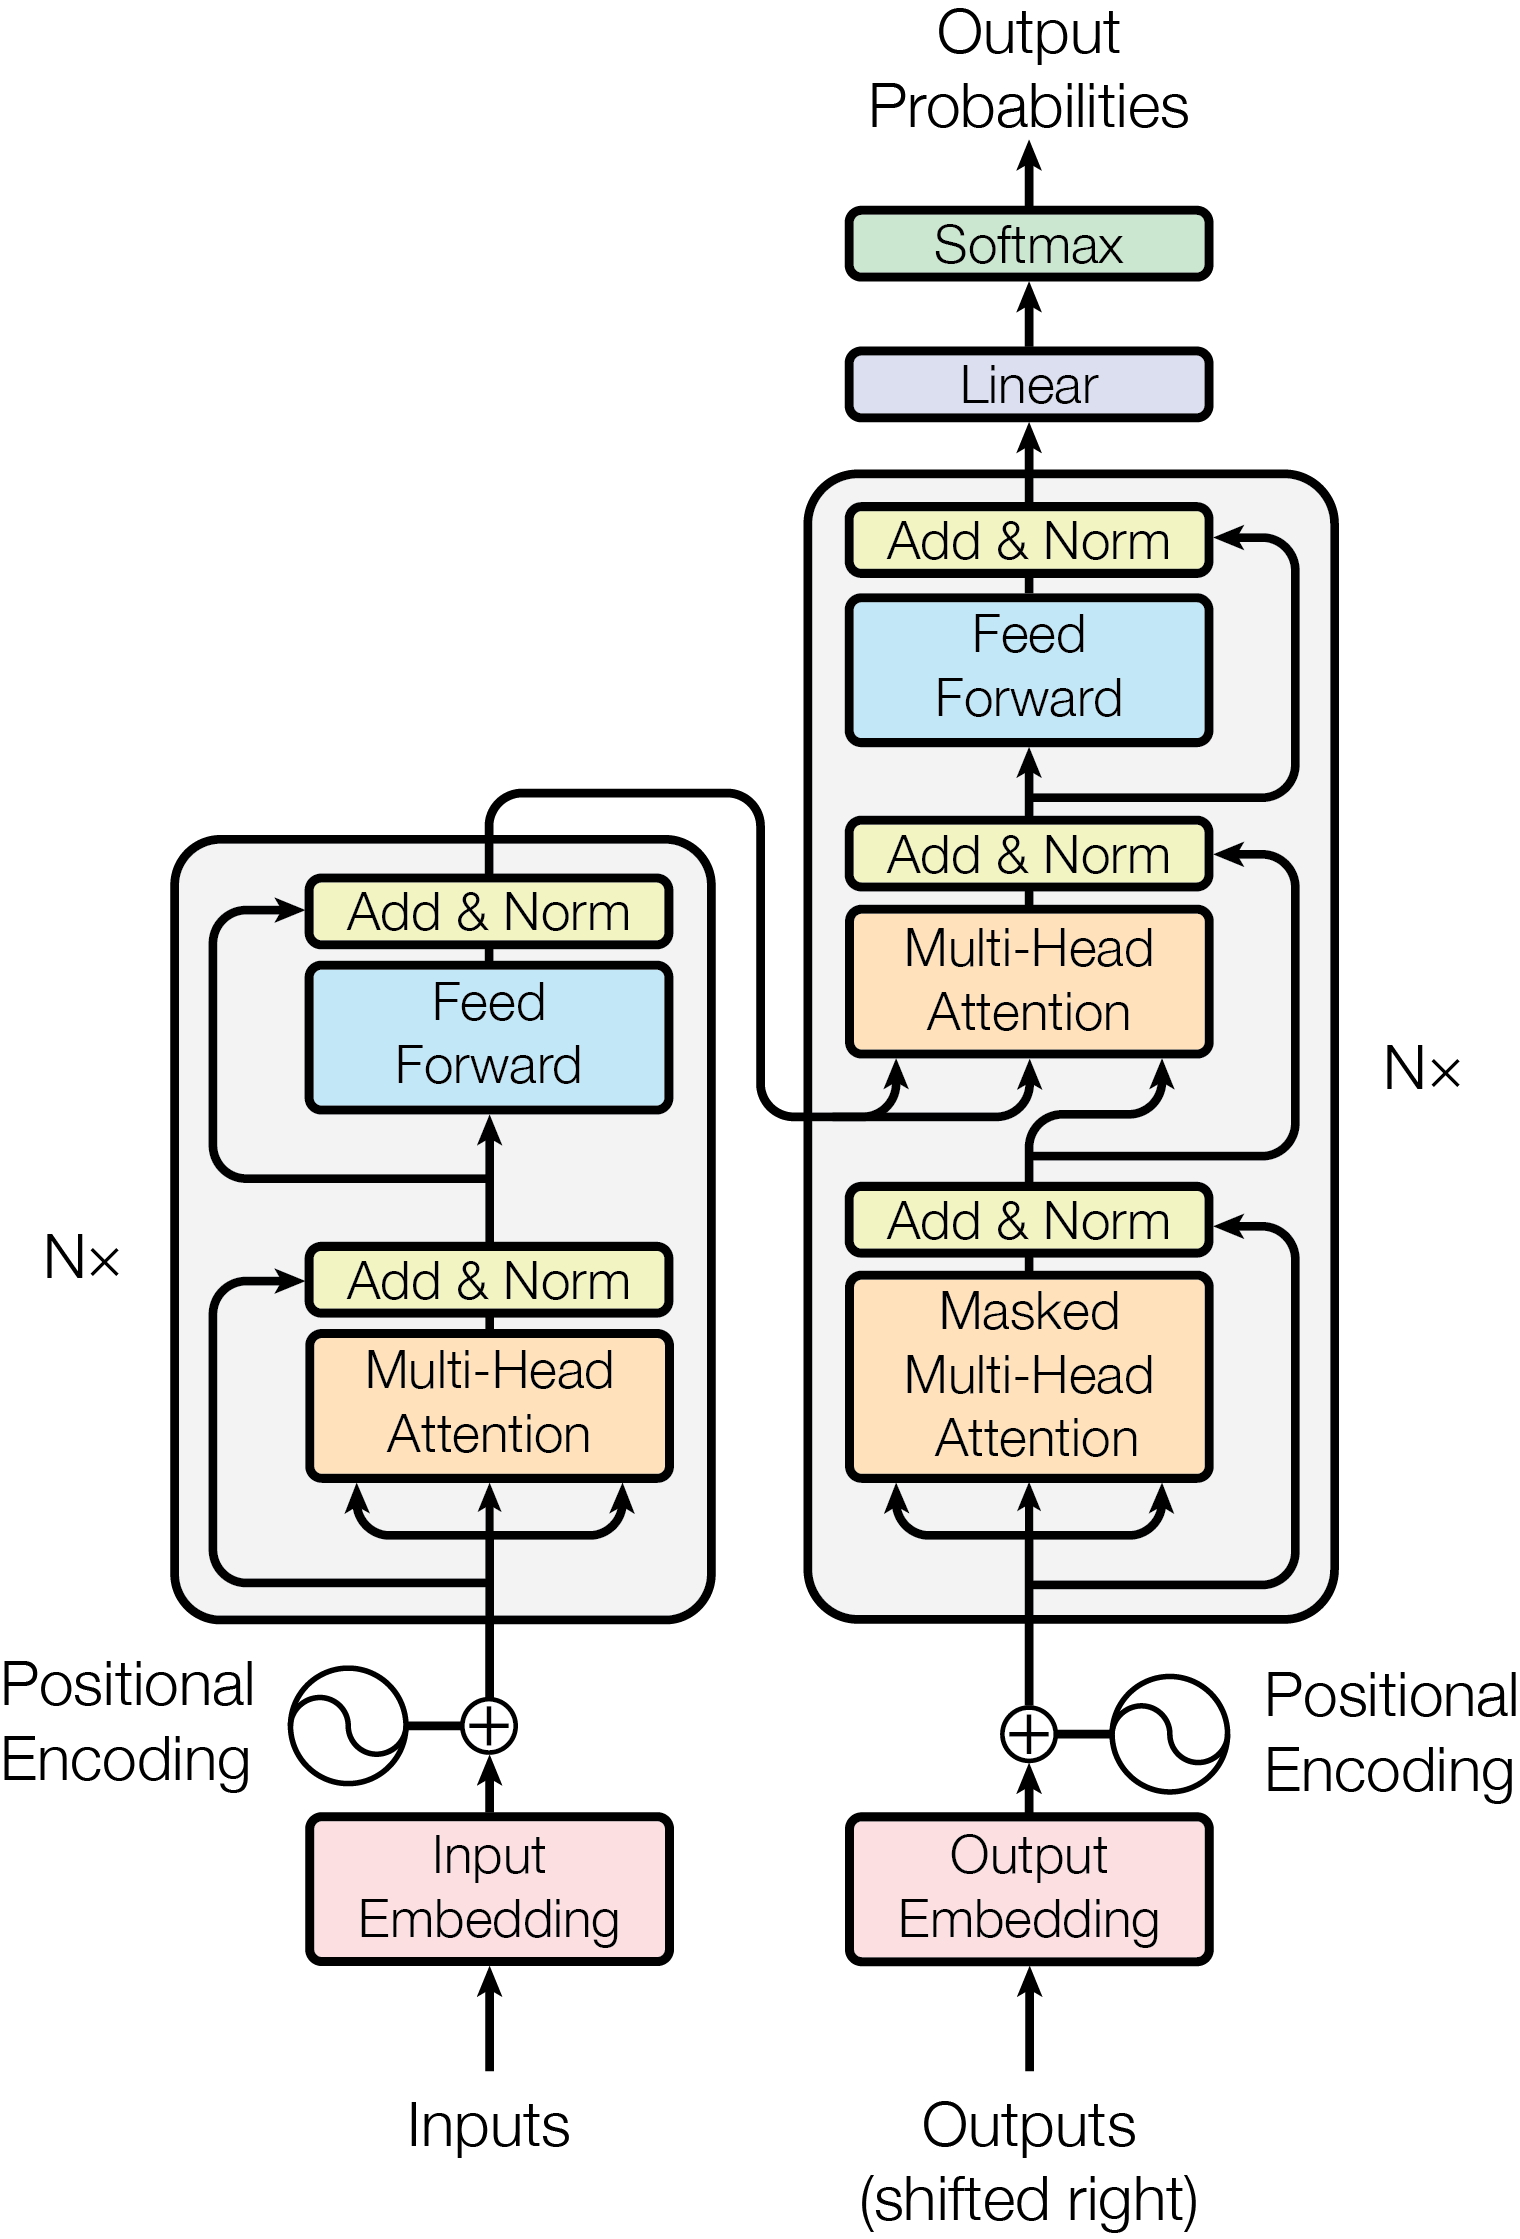
\includegraphics[width=7cm]{machine_learning/images/transformer_architecture}}
		\captionof{figure}{The original Transformer architecture \cite{NIPS2017_3f5ee243}.}
		\label{fig:machine_learning:transformer}
	\end{minipage}%
	\begin{minipage}[t]{9cm}
		\centering
		\makebox[\textwidth]{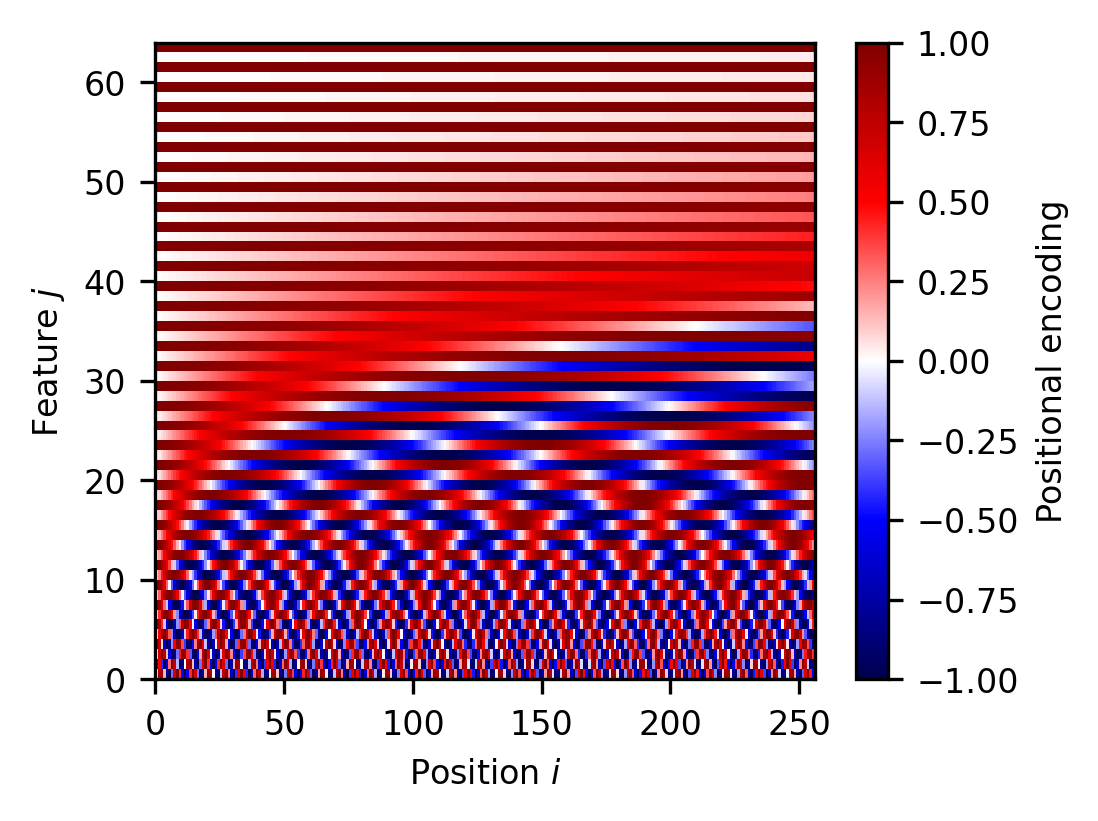
\includegraphics[width=9cm]{machine_learning/images/transformer/positional_encoding}}
		\captionof{figure}{Sinusoidal positional encodings.}
		\label{fig:machine_learning:pos_enc}
	\end{minipage}
\end{figure}

The Transformer follows an encoder--decoder architecture (see Fig.~\ref{fig:machine_learning:transformer}). The encoder processes the input sequence into an abstract representation, and the decoder  generates the output sequence from this representation. 
The decoder predicts the output sequence in an autoregressive manner, that is, token by token, starting with a beginning-of-sentence token. This makes sense for machine translation, while for other tasks the decoder can also be adapted to make predictions in parallel instead.
Modern transformer models often employ only the encoder or decoder.

Both the encoder and decoder are composed of identical stacked layers, where each layer's output is the next one's input. These layers comprise sub-layers of multi-head attention and dense networks, \emph{i.e.}\ feed-forward networks (FFNs). 

The encoder layers apply two sub-layers, self-attention followed by an FFN. The decoder layers apply three sub-layers instead: \emph{masked} self-attention, followed by cross-attention and an FFN. Masking the self-attention sub-layer ensures that the decoder can only attend to previously predicted tokens. Transformer models, which predict tokens in parallel, omit this masking. The cross-attention's source sequence is the encoder output and the target sequence is obtained from the previous sub-layer.

% residual layers
% layernorm
The architecture makes use of \emph{residual connections} for all  sub-layers, where the input is added to the output, \emph{i.e.}, $x + \text{SubLayer}(x)$. This works, since both these sub-layers return a tensor of the same dimension as the input. The FFN is,
\begin{equation}
	\text{FFN}(x) = \text{Dropout}(\text{Linear}_{d_\text{ff} \rightarrow d_\text{embed}}(\text{GELU}(\text{Linear}_{d_\text{embed} \rightarrow d_\text{ff}}(x)))),
\end{equation}
with hidden dimension $d_\text{ff}$, and a Gaussian error linear unit (GELU) activation~\cite{hendrycks2017bridging}.
Dropout~\cite{JMLR:v15:srivastava14a} is a regularization technique, which prevents networks from overfitting by randomly zeroing out elements of the given tensor. Dropout is not applied during inference.
In the original architecture, the residual connection is followed by a \emph{layer normalization}~\cite{ba2016layernormalization} to standardize the output along the embedding dimension.
This is called \emph{post}-layer normalization. To ease training, modern implementations often employ \emph{pre}-layer normalization, so $x + \text{SubLayer}(\text{LayerNorm}(x))$ instead. 

% positional encoding
Unlike in CNNs, the sequential nature of the data is not baked into the Transformer architecture itself. Thus, \emph{positional encodings} are added to encoder and decoder input tokens. The original Transformer makes use of so-called fixed sinusoidal encodings. For a token position $i<N_\text{tokens}$ and a feature $j<d_\text{embed}$, this is:  
\begin{equation}
	P(i,j) = \begin{cases}
		\sin{({i}/{N^{\frac{j}{d_\text{embed}}}})} & \text{if $j$ even,} \\
		\cos{({i}/{N^{\frac{j-1}{d_\text{embed}}}})} & \text{if $j$ odd,}
	\end{cases}
\end{equation}
where $N=\SI{E+4}{\nothing}$. See the encodings of $256$ tokens with an embedding dimension of $64$ plotted in Fig.~\ref{fig:machine_learning:pos_enc}.

%\begin{align}
%\begin{split}
%	n_1 &= \text{LayerNorm}(x) \\
%	y &= n_1 + \text{MHA}(n_1, n_1) \\
%	n_2 &= \text{LayerNorm}(y) \\
%	z &= n_2 + \text{FFN}(n_2)
%\end{split}
%\end{align}
%
%\begin{align}
%\begin{split}
%	n_1 &= \text{LayerNorm}(t) \\
%	x &= n_1 + \text{MHA}(n_1, n_1) \\
%	n_2 &= \text{LayerNorm}(x) \\
%	y &= n_2 + \text{MHA}(c, n_2) \\
%	n_3 &= \text{LayerNorm}(y) \\
%	z &= n_3 + \text{FFN}(n_3)
%\end{split}
%\end{align}

